%
% Sección de introducción a criptografía,
% Presentación de TT uno.
%
% Proyecto Lovelace.
%

\subsection{Introducción a la criptografía}

\begin{frame}{Introducción a la criptografía}{Confidencialidad}

  \begin{figure}[H]
    \begin{center}
      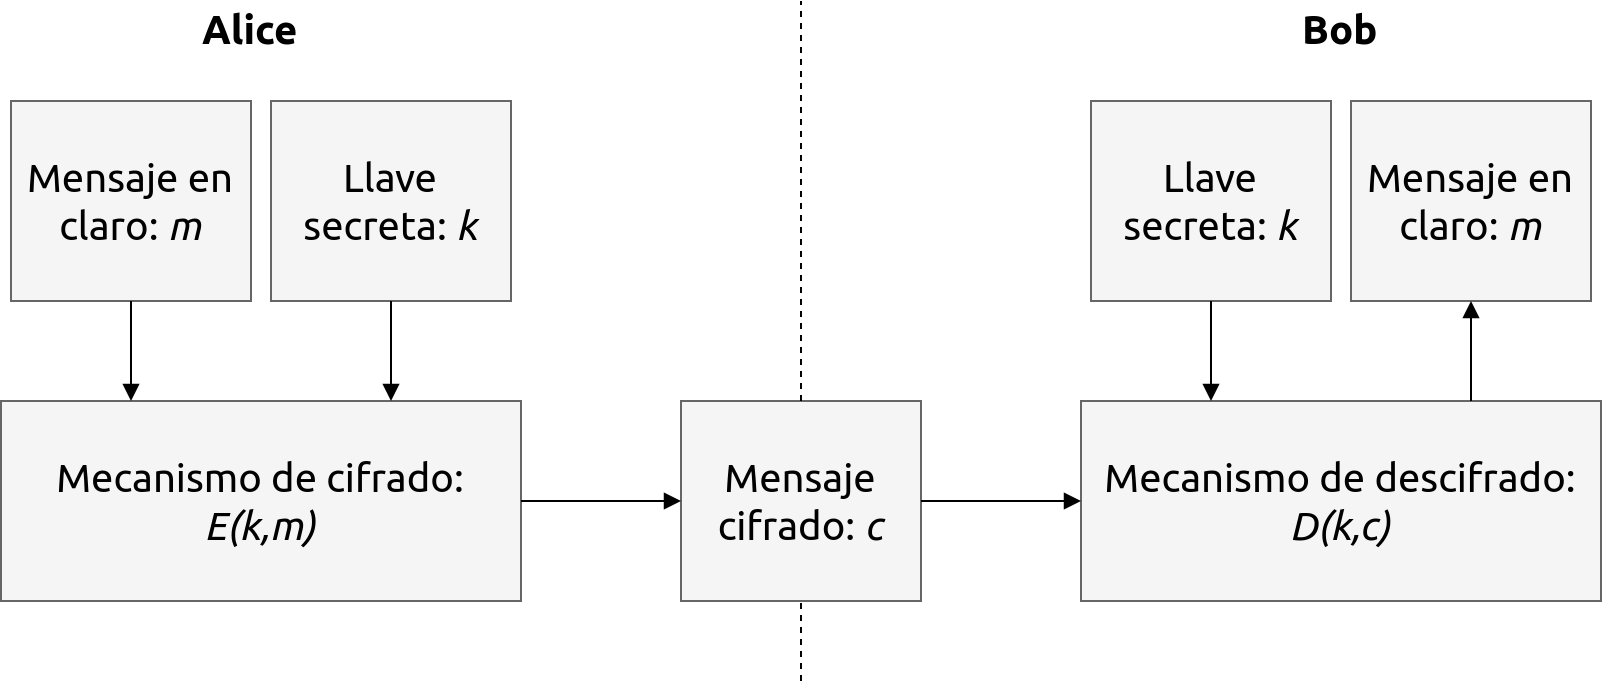
\includegraphics[width=1.0\linewidth]
        {../../../diagramas_comunes/marco_teorico/cripto_simetrica.png}
      \caption{Canal de comunicación seguro.}
    \end{center}
  \end{figure}

  \note
  {
    La idea básica de la criptografía es transformar un mensaje para que solo
    las partes autorizadas puedan leerlo. En este caso Alicia es el emisor del
    mensaje y Alberto el receptor; ambos cuentan con un secreto común: la llave.
    Alicia usa la llave y el mecanismo de cifrado para transformar su mensaje en
    algo ilegible; Alberto utiliza la llave y el mecanismo de descifrado para
    obtener el mensaje original.

    Esto se conoce como \textit{confidencialidad}, y es el principal objetivo de
    la criptografía moderna. Los otros son \textit{integridad},
    \textit{autenticación} y \textit{no repudio}.
  }

\end{frame}

